%*****************************************************
%	APPENDIX
%*****************************************************
\appendix
%-----------------------------------------------------
\chapter{Expanded Equations}
\label{app:equations}
\section{Standard Quadrotor Dynamics}
\label{app:equations.standard}
%-----------------------------------------------------
Following the fundamental 6-DOF equations of motion for a rigid body derived in Sec:\ref{subsec:dynamics.rigidbody.lagrange}, the common linearizations typically applied for generic "+" configured quadrotors are now presented. Reiterating those four differential equations, Eq:\ref{eq:states}, which describe a rigid body's motion (using rotation matrices and not quaternions):
\begin{subequations}
\begin{equation}
\dot{\vec{\mathcal{E}}}=\mathbb{R}_b^I(-\eta)\vec{v}_b~~~~\in\mathcal{F}^I
\end{equation}
\vspace{-10pt}
\begin{equation}\label{eq:app-position}
\dot{\vec{v}}_b=m_b^{-1}\big[-\vec{\omega}_b\times m_b\vec{v}_b+m_b\mathbb{R}_I^b(-\eta)\vec{G}_I+\vec{F}_{net}\big]~~~~\in\mathcal{F}^b
\end{equation}
\vspace{-5pt}
\begin{equation}\label{eq:app-euler}
\dot{\vec{\eta}}=\Phi(\eta)\vec{\omega}_b~~~~\in\mathcal{F}^{v2},\mathcal{F}^{v1},\mathcal{F}^I
\end{equation}
\vspace{-10pt}
\begin{equation}\label{eq:app-attitude}
\dot{\vec{\omega}}_b=J_b^{-1}\big[-\vec{\omega}_b\times J_b\vec{\omega}_b+\vec{\tau}_{net}\big]~~~~\in\mathcal{F}^b
\end{equation}
\end{subequations}
With the Euler matrix, $\Phi(\eta)$, defined in Eq:\ref{eq:angular-rates.f}. The net heave thrust produced by motors $i\in[1:4]$, bound perpendicularly to the $\hat{Z}_b$ axis, is given by:
\begin{subequations}
\begin{equation}
\vec{T}=\sum_{i=1}^4F(\Omega_i)\cdot\hat{Z}_b~~~~\in\mathcal{F}^b
\end{equation}
The simplified relationship between the thrust scalar $T(\Omega_i)$ and the propeller's rotational speed $\Omega_i$ in $[\text{RPS}]$ is approximately quadratic:
\begin{equation}
F(\Omega_i)\approx k_1\Omega_i^2
\end{equation}
\end{subequations}
Similarly the aerodynamic torque opposing each rotating propeller, about the propellers $\hat{Z}_b$ axis, is:
\begin{equation}
Q(\Omega_i)\approx k_2\Omega_i^2
\end{equation}
Coefficients $k_1$ \& $k_2$ are typically determined from physical thrust tests. The controllable pitch and roll torques, $\tau_\phi$ \& $\tau_\theta$ about the $\hat{X}_b$ and $\hat{Y}_b$ axes respectively, are generated by opposing differential lift forces. Lastly the yaw torque, $\tau_\psi$ about the $\hat{Z}_b$ axis, is generated only a net response to the rotational aerodynamic propeller torques. The control torque inputs are then defined as:
\begin{subequations}
\begin{equation}
\tau_{\phi}=L_{arm}\big(F(\Omega_1)-F(\Omega_3)\big)\cdot\hat{X}_b
\end{equation}
\vspace{-10pt}
\begin{equation}
\tau_{\theta}=L_{arm}\big(F(\Omega_2)-F(\Omega_4)\big)\cdot\hat{Y}_b
\end{equation}
\vspace{-10pt}
\begin{equation}
\tau_{\psi}=\sum_{i=1}^4(-1)^{i}Q(\Omega_i)\cdot\hat{Z}_b
\end{equation}
\end{subequations}
\par
Then expanding the translational position and attitude state differentials, Eq:\ref{eq:app-position} \& Eq:\ref{eq:app-attitude}, to their component forms (assuming the vehicle's inertial matrix $J_b$ is diagonal):
\begin{subequations}\label{eq:app-states}
\begin{equation}
\begin{pmatrix}
\dot{u}\\
\dot{v}\\
\dot{w}
\end{pmatrix}
=
\begin{pmatrix}
rv-qw\\
pw-ru\\
qu-pv
\end{pmatrix}
+
\begin{pmatrix}
-g sin(\theta)\\
g cos(\theta)sin(\phi)\\
g cos(\theta)cos(\phi)
\end{pmatrix}
+
\frac{1}{m}\begin{pmatrix}
0\\
0\\
T
\end{pmatrix}
~~~~\in\mathcal{F}^b
\end{equation}
\vspace{-5pt}
\begin{equation}
\begin{pmatrix}
\dot{p}\\
\dot{q}\\
\dot{r}
\end{pmatrix}
=\begin{pmatrix}
\frac{J_{yy}-J_{zz}}{J_{xx}}qr\\
\frac{J_{zz}-J_{xx}}{J_{yy}}pr\\
\frac{J_{xx}-J_{yy}}{J_{zz}}pq
\end{pmatrix}
+
J_b^{-1}\begin{pmatrix}
\tau_\phi\\
\tau_\theta\\
\tau_\psi
\end{pmatrix}~~~~\in\mathcal{F}^b
\end{equation}
\end{subequations}
Considering the size of a typical angular rate, $\vec{\omega}_b\approx\vec{0}$; the gyroscopic and Coriolis effects on the body (namely both cross product terms) are sufficiently small enough to be regarded as negligible. Assuming too that the body has a (\emph{roughly}) diagonal inertial matrix. Then the following holds true around the origin when $\vec{\omega}_b\approx\vec{0}$:
\begin{equation}
\begin{pmatrix}
rv-qw\\
pw-ru\\
qu-pv
\end{pmatrix}
\approx
\vec{0}
~~~\text{and}~~~
=\begin{pmatrix}
\frac{J_{yy}-J_{zz}}{J_{xx}}qr\\
\frac{J_{zz}-J_{xx}}{J_{yy}}pr\\
\frac{J_{xx}-J_{yy}}{J_{zz}}pq
\end{pmatrix}
\approx
\vec{0}
\end{equation}
As a result, state differentials in Eq:\ref{eq:app-states} can then reduce to the following:
\begin{equation}
\begin{pmatrix}
\dot{u}\\
\dot{v}\\
\dot{w}
\end{pmatrix}
=
\begin{pmatrix}
-g sin(\theta)\\
g cos(\theta)sin(\phi)\\
g cos(\theta)cos(\phi)
\end{pmatrix}
+
\frac{1}{m}\begin{pmatrix}
0\\
0\\
T
\end{pmatrix}
~~~\text{and}~~~
\begin{pmatrix}
\dot{p}\\
\dot{q}\\
\dot{r}
\end{pmatrix}
=
\begin{pmatrix}
\frac{1}{\mathbb{I}_x}\tau_\phi\\
\frac{1}{\mathbb{I}_y}\tau_\theta\\
\frac{1}{\mathbb{I}_z}\tau_\psi
\end{pmatrix}
\end{equation}
Similarly, at an attitude near to the origin and at hovering conditions the following simplification applies to the Euler matrix $\Phi(\eta)$:
\begin{equation}
\Phi(\eta)\approx\vec{1}~~\text{for}~~\eta\approx\vec{0}
\end{equation}
And so from Eq:\ref{eq:app-euler} the body's \emph{Euler rates} are approximately equivalent to its angular velocity:
\begin{equation}\label{eq:app-euler-approx}
\begin{pmatrix}\dot{p}&\dot{q}&\dot{r}\end{pmatrix}^T\approx\begin{pmatrix}\ddot{\phi}&\ddot{\theta}&\ddot{\psi}\end{pmatrix}^T
\Rightarrow
\dot{\eta}\approx\omega_b
\end{equation}
The above Eq:\ref{eq:app-euler-approx} is not an insignificant result. The difficulty with Euler angle parameterization for body attitude is that each Euler angle is defined with respect to a sequential reference frame, Eq:\ref{eq:angular-rates-eq}. As such, the state equations for Eq:\ref{eq:app-states} then reduce to the following six SISO controllable plants when the vehicle's angular velocity is small:
\begin{subequations}\label{eq:app-simplified}
\begin{equation}
\ddot{x}=(-cos(\phi)sin(\theta)cos(\psi)-sin(\phi)sin(\psi)\frac{1}{m}T
\end{equation}
\vspace{-5pt}
\begin{equation}
\ddot{y}=(-cos(\phi)sin(\theta)sin(\psi)+sin(\phi)cos(\psi))\frac{1}{m}T
\end{equation}
\vspace{-5pt}
\begin{equation}
\ddot{z}=g-(cos(\phi)cos(\theta)\frac{1}{m}T
\end{equation}
\vspace{-7pt}
\begin{equation}
\ddot{\phi}=\frac{1}{J_{xx}}\tau_\phi
\end{equation}
\vspace{-7pt}
\begin{equation}
\ddot{\theta}=\frac{1}{J_{yy}}\tau_\theta
\end{equation}
\vspace{-7pt}
\begin{equation}
\ddot{\psi}=\frac{1}{J_{zz}}\tau_\psi
\end{equation}
\end{subequations}
Typically, the simplified Eq:\ref{eq:app-simplified} is abstracted to an "augmented pilot control system". In such a case the controllable inputs are abstracted to $T,~\ddot{\phi},~\ddot{\theta},~\ddot{\psi}$. Wherein the pilot dictates the attitude torques and net heave thrust for the quadrotor, mostly with various flavours of PD control for each channel.
\newpage
%-----------------------------------------------------
\section{Blade-Element Momentum Expansion}
\label{app:equations.bem} 
%-----------------------------------------------------
Expanding on the Blade-Element Momentum equations from Eq:\ref{eq:moment-thrust-element} and Eq:\ref{eq:bem-thrust}. Reiterating the integral equations, they are:
\begin{subequations}
\begin{equation}\label{eq:app-bem-thrust}
dT=\rho 4\pi r v_\infty(1+a)a.dr
\end{equation}
\vspace{-10pt}
\begin{equation}\label{eq:app-bem-torque}
dT = \frac{1}{2} a_L b c \rho (\Omega r)^2\big(\theta-\frac{v_\infty+v_i}{\Omega r}\big).dr
\end{equation}
\end{subequations}
Both Eq:\ref{eq:app-bem-thrust}-\ref{eq:app-bem-torque} are integrals taken accross the length of the propeller blade. Equating the two and defining an inflow ratio term $\lambda=\frac{v_\infty+v_i}{\Omega r}=\frac{v_\infty(1+a)}{\Omega r}$ yields the following quadratic equation:
\begin{equation}\label{eq:app-bem-quadratic}
\lambda^2+\bigg(\frac{\sigma a_L}{8}+\lambda_c\bigg)\lambda-\frac{\sigma a_L}{8}\theta\frac{r}{R}=0
\end{equation}
Where $\lambda_c$ is the nominal free-stream inflow ratio when $v_i=0$. Another term, $\sigma$, is defined as the propeller solidity and is given by:
\begin{equation}
\sigma = \frac{bc}{\pi R}
\end{equation}
Then, solving Eq:\ref{eq:app-bem-quadratic} for $\lambda$:
\begin{equation}
\lambda=\sqrt{\bigg(\frac{\sigma a_L}{16}-\frac{\lambda_c}{2}\bigg)^2+\frac{\sigma a_L}{8}\theta\frac{r}{R}}-\bigg(\frac{\sigma a_L}{16}-\frac{\lambda_c}{2}\bigg)
\end{equation}
So then the inflow ratio can be solved as a function of the propeller element's aerofoil profile and its static inflow factor. In static conditions, the inflow factor is:
\begin{equation}
\lambda=\frac{v_i}{\Omega r} = \sqrt{\frac{C_{T0}}{2}}
\end{equation}
Then substituting $\lambda$ back into Eq:\ref{eq:bem-thrust} and solving the integral produces an instantaneous thrust value. The difficulty of solving the blade-element momentum integrals is knowing the exact chord profile and local angle of attack.
%-----------------------------------------------------
\section{Euler-Angles from Quaternions}
\label{app:equations.quaternions}
%-----------------------------------------------------
The solution for Euler angles from an attitude quaternion is an easy trigonometric inversion. Noting that the transformation from the body frame to each motor frame follows the Z-Y-X sequence,and using an inversion solution adapted from \cite{computingeuler}, where the transformation to quaternions is based on Shoemake's\cite{shoemake} definition. Each quaternion can be constructed from sequenced Euler angles, as in Eq:\ref{eq:quaternion-sequence}.
Then, solving for each euler angle using simultaneous solutions and inverse trigonometry:
\begin{equation}\label{eq:app-quaternion-eule}
\begin{bmatrix}
\phi\\
\theta\\
\psi
\end{bmatrix}
=
\begin{bmatrix}
arctan2\big(2(q_0q_x+q_yq_z),~1-2(q_x\text{}^2+q_y\text{}^2)\big)\\
arcsin\big(2(q_0q_y-q_xq_z)\big)\\
arctan2\big(2(q_0q_z+q_xq_y),~1-2(q_y\text{}^2+q_z\text{}^2)\big)
\end{bmatrix}
\end{equation}
%-----------------------------------------------------
\chapter{Design Bill of Materials}
\label{app:bom}
%-----------------------------------------------------
\section{Parts List}
%-----------------------------------------------------
\begin{table}[htbp]
\centering
\begin{tabularx}{\textwidth}{|X|l|l|}
\hline
\multicolumn{1}{|c|}{Part Name} & No. Used & Unit Weight[g]\\ \hline
\multicolumn{3}{|c|}{Electronics}\\ \hline
SPRacing F3 Deluxe Flight Controller & 1 & 8\\ \hline
OrangeRx 615X 2.4 GHz 6CH Receiver & 1 & 9.8\\ \hline
Signal Converter SBUS-PPM-PWM & 1 & 5.0\\ \hline 
STLink-V2 Debugger & 1 & 3\\ \hline
RotorStar Super Mini S-BEC 10A & 1 & 30\\ \hline
128x96" OLED Display & 1 & 7 \\ \hline
XBee-Pro S1 & 2 & 4 \\ \hline
HobbyWing XRotor 20A Opto ESC & 4 & 15\\ \hline
OrangeRX RPM Sensor & 4 & 2\\ \hline
HobbyKing Multi-Rotor Power Distribution Board & 1 & 49\\ \hline
\multicolumn{3}{|c|}{Motors}\\ \hline
Corona DS-339MG & 8 & 32\\ \hline
Cobra 2208 2000KV Brushlesss DC & 4 & 44.2\\ \hline
\multicolumn{3}{|c|}{Frame Components}\\ \hline
APM Flight Controller Damping Platform & 1 & 7\\ \hline
HobbyKing SK450 Replacement Arm (2 pcs) & 2 & 51\\ \hline
SK450 Extended Landing Skid & 1 & 23.25\\ \hline
Alloy Servo Arm (FUTABA) & 8 & 4\\ \hline
10X18X6 Radial Ball Bearing & 8 & 5\\ \hline
80g Damping Ball & 32 & $\approx 0$\\ \hline
Plastic Retainers for Damping Balls & 32 & $\approx 0$\\ \hline
3/5mm Aluminum Prop Adapter & 4 & $\approx 1$\\ \hline
6x4.5 Gemfam 3-Blade Propeller & 4 & 6\\ \hline
M3 6mm Hex Nylon Spacer & 8 & $\approx 0$\\ \hline
M3 16mm Hex Nylon Spacer & 32 & $\approx 0$\\ \hline
M3 25mm Nylon Screw & 128 & $\approx 0.08$\\ \hline
M2.5x10mm Socket Head Cap Screw & 36 & $\approx 0.2$\\ \hline
M2.5x25mm Socket Head Cap Screw & 20 & $\approx 0.6$\\ \hline
M2.5 A-Lok Nut & 16 & $\approx 0$\\ \hline 
\end{tabularx}
\label{tab:partslist}
\caption{Parts List}
\end{table}
%-----------------------------------------------------
\newpage
%-----------------------------------------------------
\newgeometry{left=1cm,right=1cm,top=2cm,bottom=2cm}
\begin{figure}[hbtp]
\vspace{-20pt}
\centering
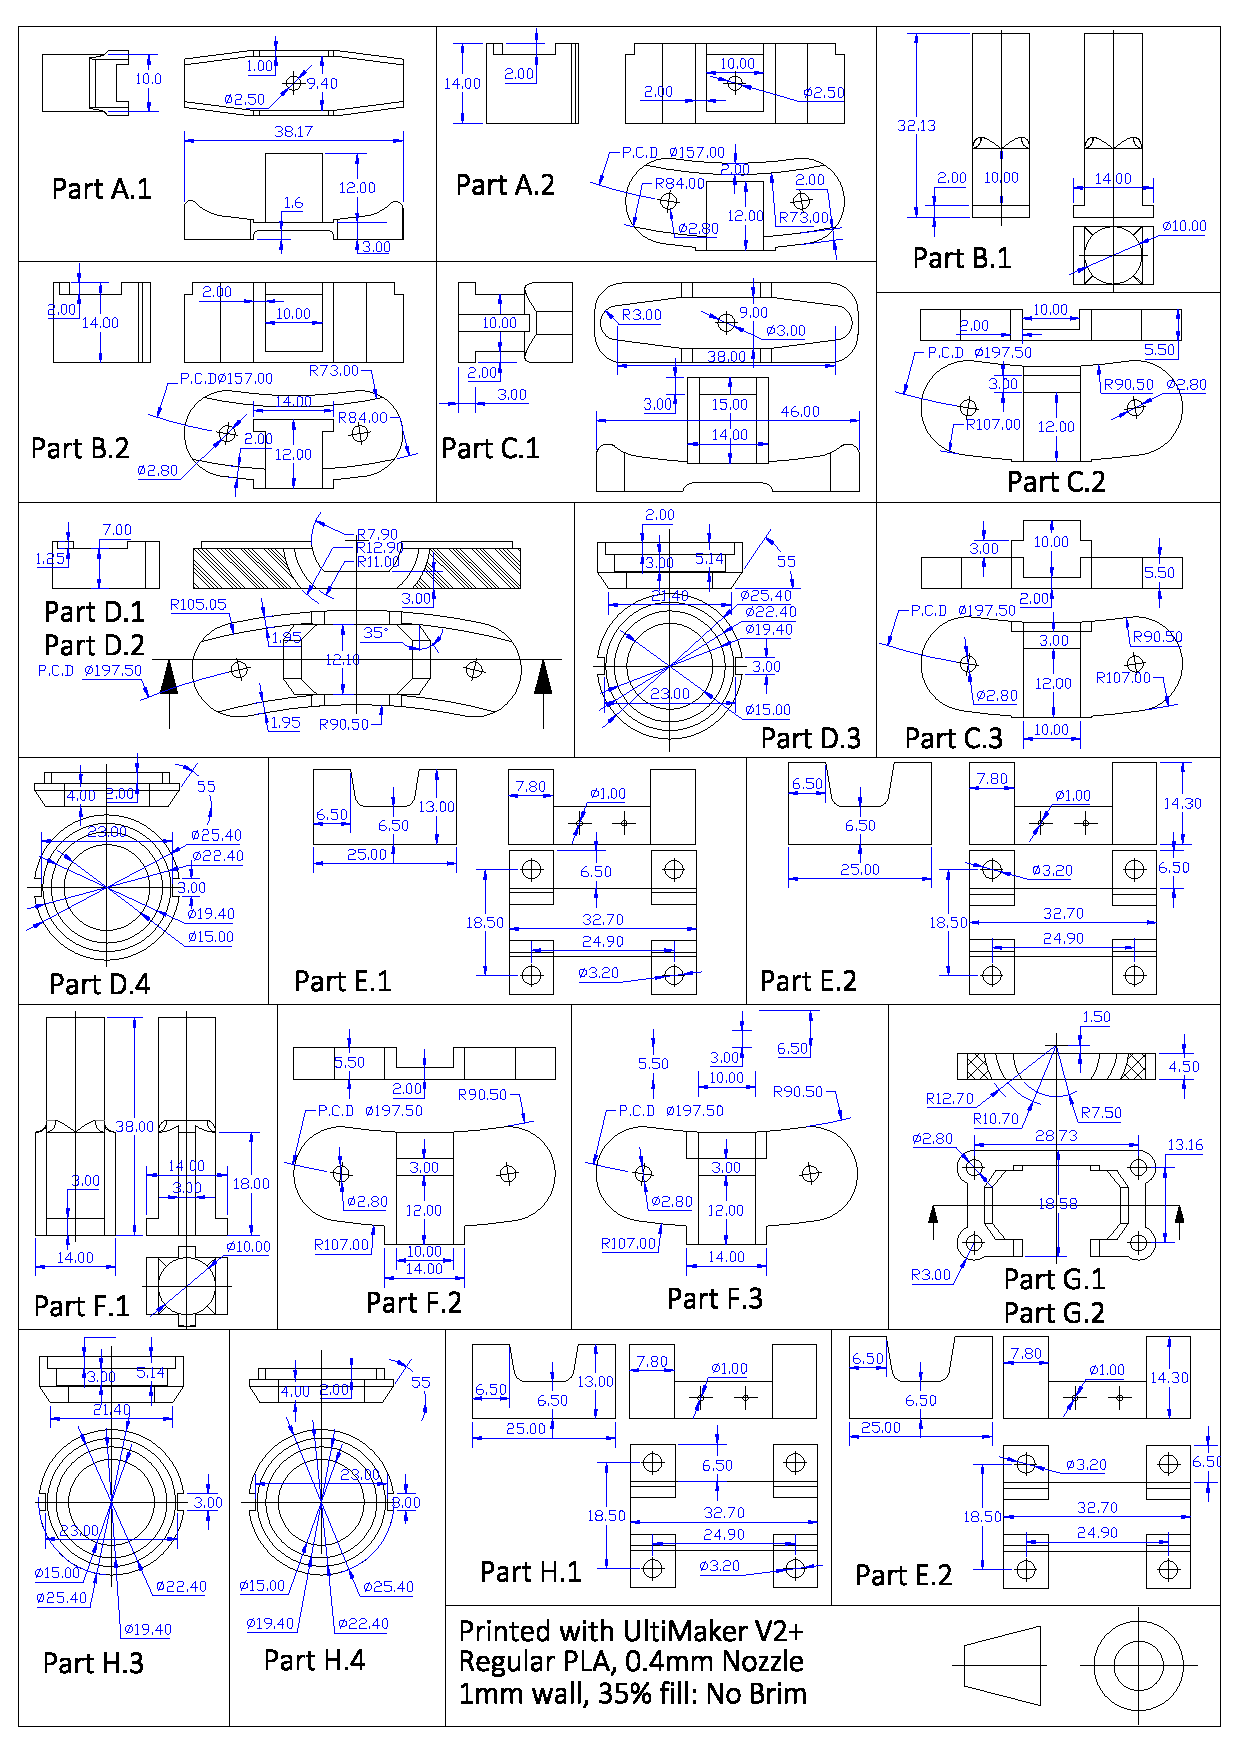
\includegraphics[width=0.98\textwidth]{pdfpages/working.pdf}
\captionof{table}{3D Printed Parts}
\end{figure}
\restoregeometry
%-----------------------------------------------------
\newpage
%-----------------------------------------------------
\newgeometry{left=1cm,right=1cm,top=2cm,bottom=1cm}
\begin{table}[htbp]
\label{tab:damping-assemblies.a}
\centering
\begin{tabularx}{\textwidth}{|X|X|}
\hline
\multicolumn{2}{|c|}{Bracket Assemblies 2}\\
\hline
\begin{minipage}{0.5\textwidth}
\vspace{6pt}
\centering
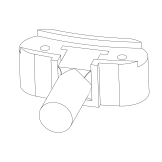
\includegraphics[width=0.7\textwidth]{figs/appendix/assembly-inner-bearing}
\captionof{figure}{Bearing Bracket Inner Ring Assembly}
Parts: A.1, A.2
\end{minipage}
&
\begin{minipage}{0.5\textwidth}
\vspace{6pt}
\centering
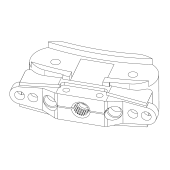
\includegraphics[width=0.7\textwidth]{figs/appendix/assembly-inner-servo}
\captionof{figure}{Servo Bracket Inner Ring Assembly}
Parts: B.1, B.2, M3 Servo Horn
\end{minipage}
\\
\hline
\begin{minipage}{0.5\textwidth}
\vspace{6pt}
\centering
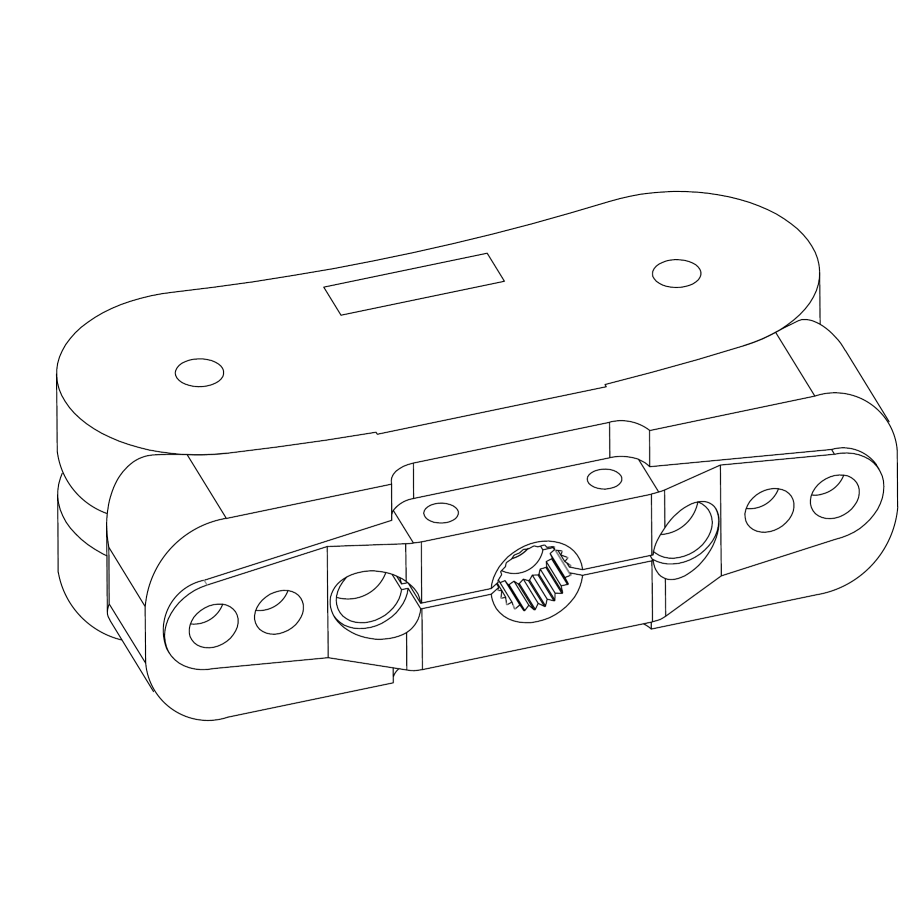
\includegraphics[width=0.7\textwidth]{figs/appendix/assembly-middle-servo-bracket}
\captionof{figure}{Servo Bracket Middle Ring Assembly}
Parts: C.1, C.2, C.3, M3 Servo Horn
\end{minipage}
&
\begin{minipage}{0.5\textwidth}
\vspace{6pt}
\centering
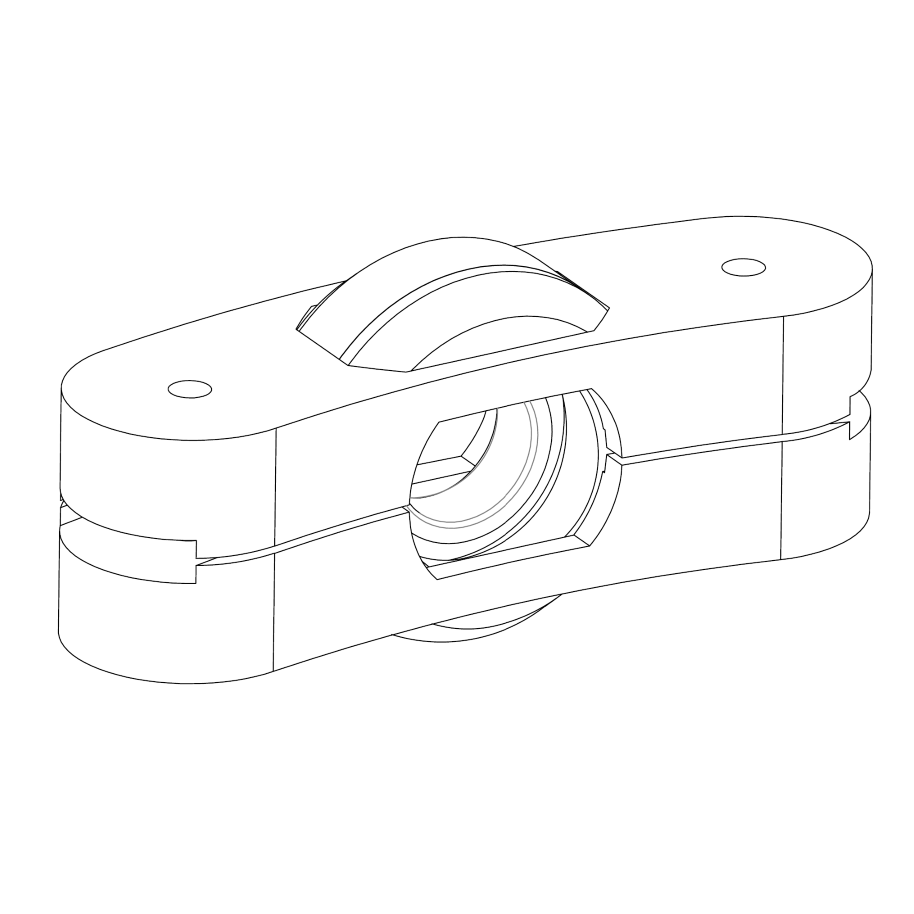
\includegraphics[width=0.7\textwidth]{figs/appendix/assembly-middle-bearing-holder}
\captionof{figure}{Bearing Holder Middle Ring Assembly}
Parts: D.1, D.2, D.3, D.4, 18-10 Bearing
\end{minipage}
\\
\hline
\begin{minipage}{0.5\textwidth}
\vspace{6pt}
\centering
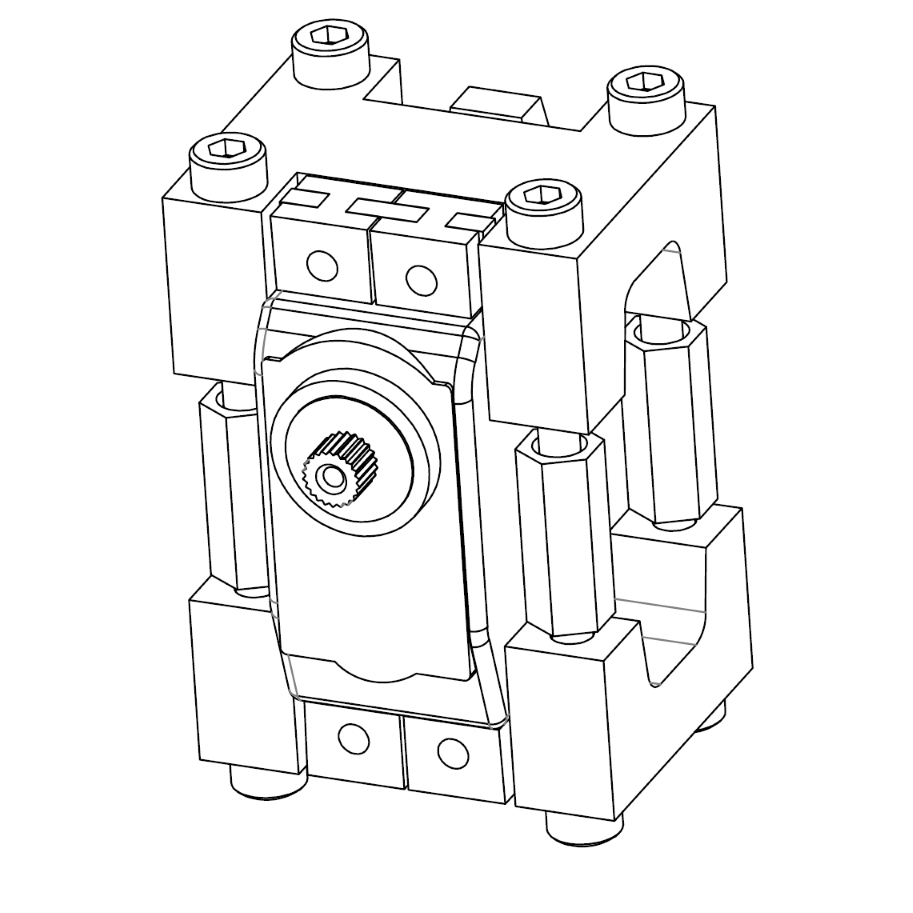
\includegraphics[width=0.7\textwidth]{figs/appendix/assembly-middle-servo-mount}
\captionof{figure}{Servo Mount Middle Ring Assembly}
Parts: E.1, E.2, Corona Servo \& Fasteners
\end{minipage}
&
\begin{minipage}{0.5\textwidth}
\vspace{6pt}
\centering
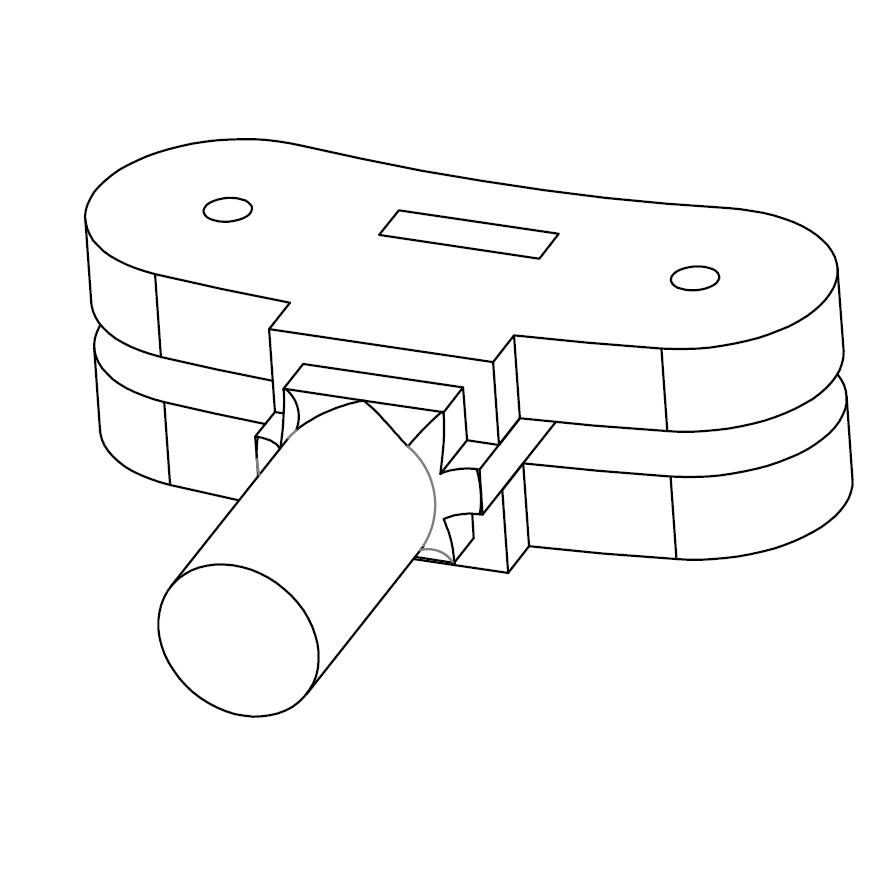
\includegraphics[width=0.7\textwidth]{figs/appendix/assembly-middle-bearing-bracket}
\captionof{figure}{Bearing Shaft Middle Ring Assembly}
Parts: F.1, F.2, F.3
\end{minipage}
\\
\hline
\end{tabularx}
\caption{Inner \& Middle Ring Assemblies}
\end{table}
\restoregeometry
%-----------------------------------------------------
\newpage
%-----------------------------------------------------
% Table 2
\newgeometry{left=1cm,right=1cm,top=2cm,bottom=0.5cm}
\begin{table}[htbp]
\label{tab:damping-assemblies.b}
\centering
\begin{tabularx}{\textwidth}{|X|X|}
\hline
\multicolumn{2}{|c|}{Bracket Assemblies 2}\\
\hline
\begin{minipage}{0.5\textwidth}
\vspace{6pt}
\centering
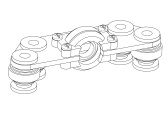
\includegraphics[width=0.7\textwidth]{figs/appendix/assembly-damping-bearing}
\captionof{figure}{Bearing Holder Damping Assembly}
Parts: G.1, G.2, G.3, G.4, 18-10 Bearing, 80g 
\\
Damping Balls, Bearing Holder Damping Bracket
\end{minipage}
&
\begin{minipage}{0.5\textwidth}
\vspace{6pt}
\centering
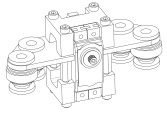
\includegraphics[width=0.7\textwidth]{figs/appendix/assembly-damping-servo}
\captionof{figure}{Servo Mount Damping Assembly}
Parts: H.1, H.2, Corona Servo \& Fasteners, 80g Damping Balls, Servo Mount Damping Bracket
\end{minipage}
\\
\hline
\end{tabularx}
\caption{Damping Assemblies}
\end{table}
\par
\begin{table}[htbp]
\label{tab:damping-backets}
\centering
\begin{tabularx}{\textwidth}{|X|X|}
\hline
\multicolumn{2}{|c|}{Laser Cut Brackets}\\
\hline
\begin{minipage}{0.5\textwidth}
\vspace{6pt}
\centering
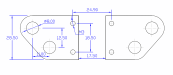
\includegraphics[width=0.8\textwidth]{figs/appendix/damping-bracket-servo}
\captionof{figure}{Servo Mount Damping Bracket}
\end{minipage}
&
\begin{minipage}{0.5\textwidth}
\vspace{6pt}
\centering
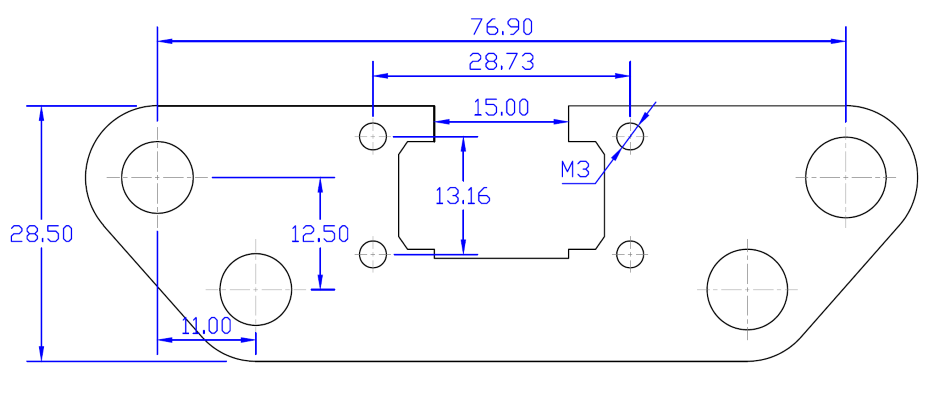
\includegraphics[width=0.8\textwidth]{figs/appendix/damping-bracket-bearing}
\captionof{figure}{Bearing Holder Damping Bracket}
\end{minipage}
\\
\hline
\begin{minipage}{0.5\textwidth}
\vspace{12pt}
\centering
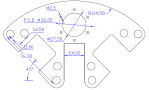
\includegraphics[width=0.9\textwidth]{figs/appendix/damping-arm-mount}
\captionof{figure}{Arm Mount Damping Bracket}
\end{minipage}
&
\begin{minipage}{0.5\textwidth}
\vspace{6pt}
\centering
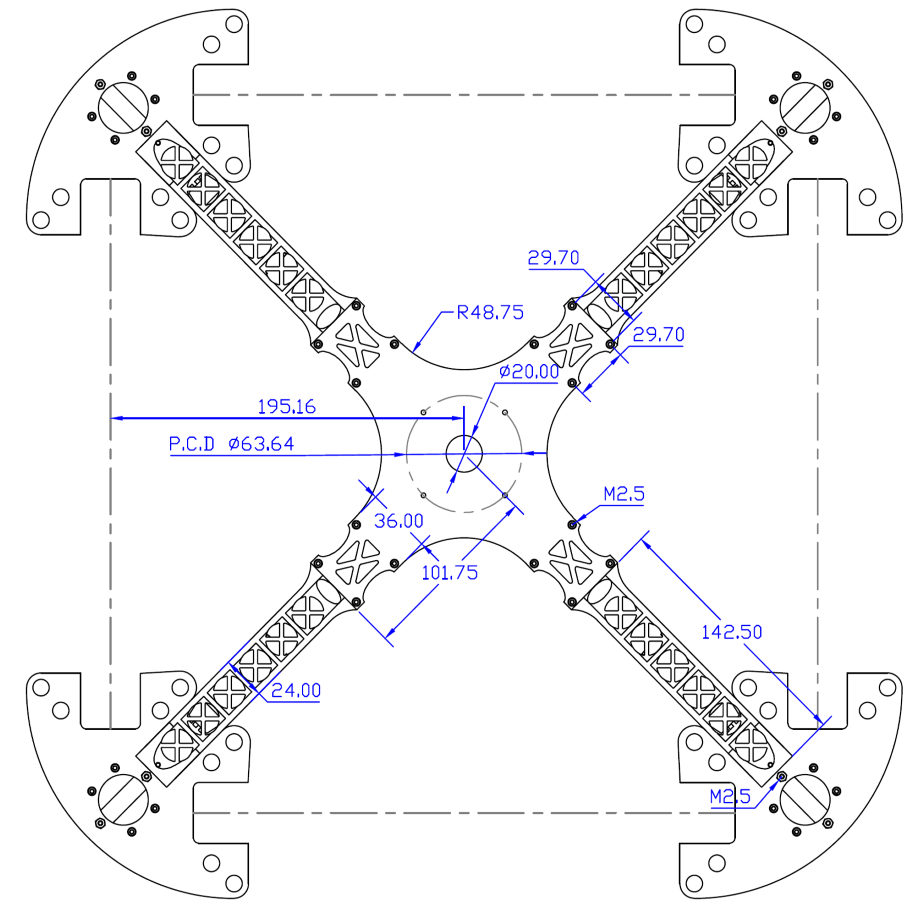
\includegraphics[width=0.6\textwidth]{figs/appendix/frame-assembly}
\captionof{figure}{Frame Brackets}
\end{minipage}
\\
\hline
\end{tabularx}
\caption{Laser Cut Damping Brackets}
\end{table}

\restoregeometry
%-----------------------------------------------------
\newpage
%-----------------------------------------------------
\newgeometry{left=1cm,right=1cm,top=2cm,bottom=1cm}
\vspace{-20pt}
\begin{figure}[hbtp]
\centering
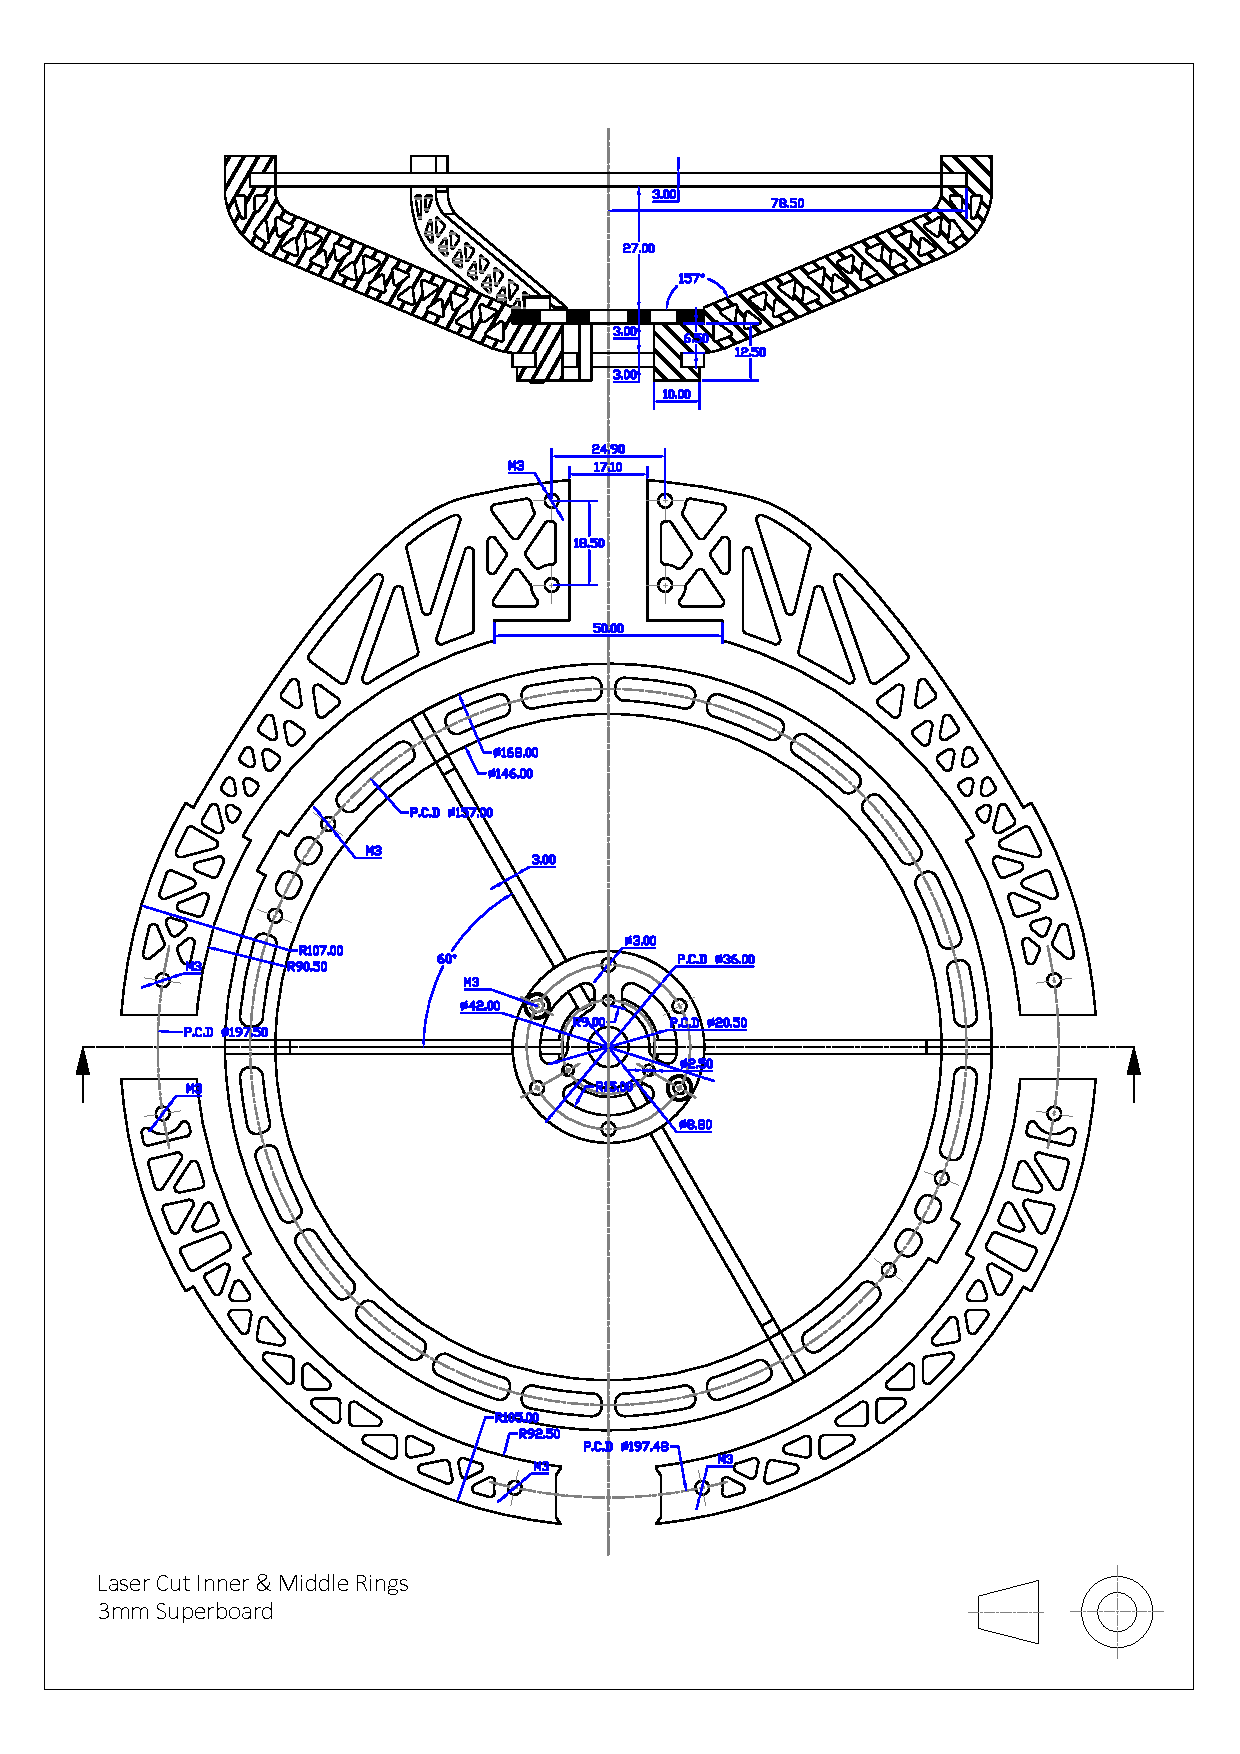
\includegraphics[width=0.95\textwidth]{pdfpages/rings.pdf}
\captionof{table}{Laser Cut Parts}
\end{figure}
\restoregeometry
%-----------------------------------------------------
\newpage
%-----------------------------------------------------
\newgeometry{left=1cm,right=1cm,top=2cm,bottom=1cm}
\section{F3 Deluxe Schematic Diagram}
\label{app:deluxe-diagram}
{\centering
\fbox{
\begin{minipage}{0.9\textwidth}
\centering
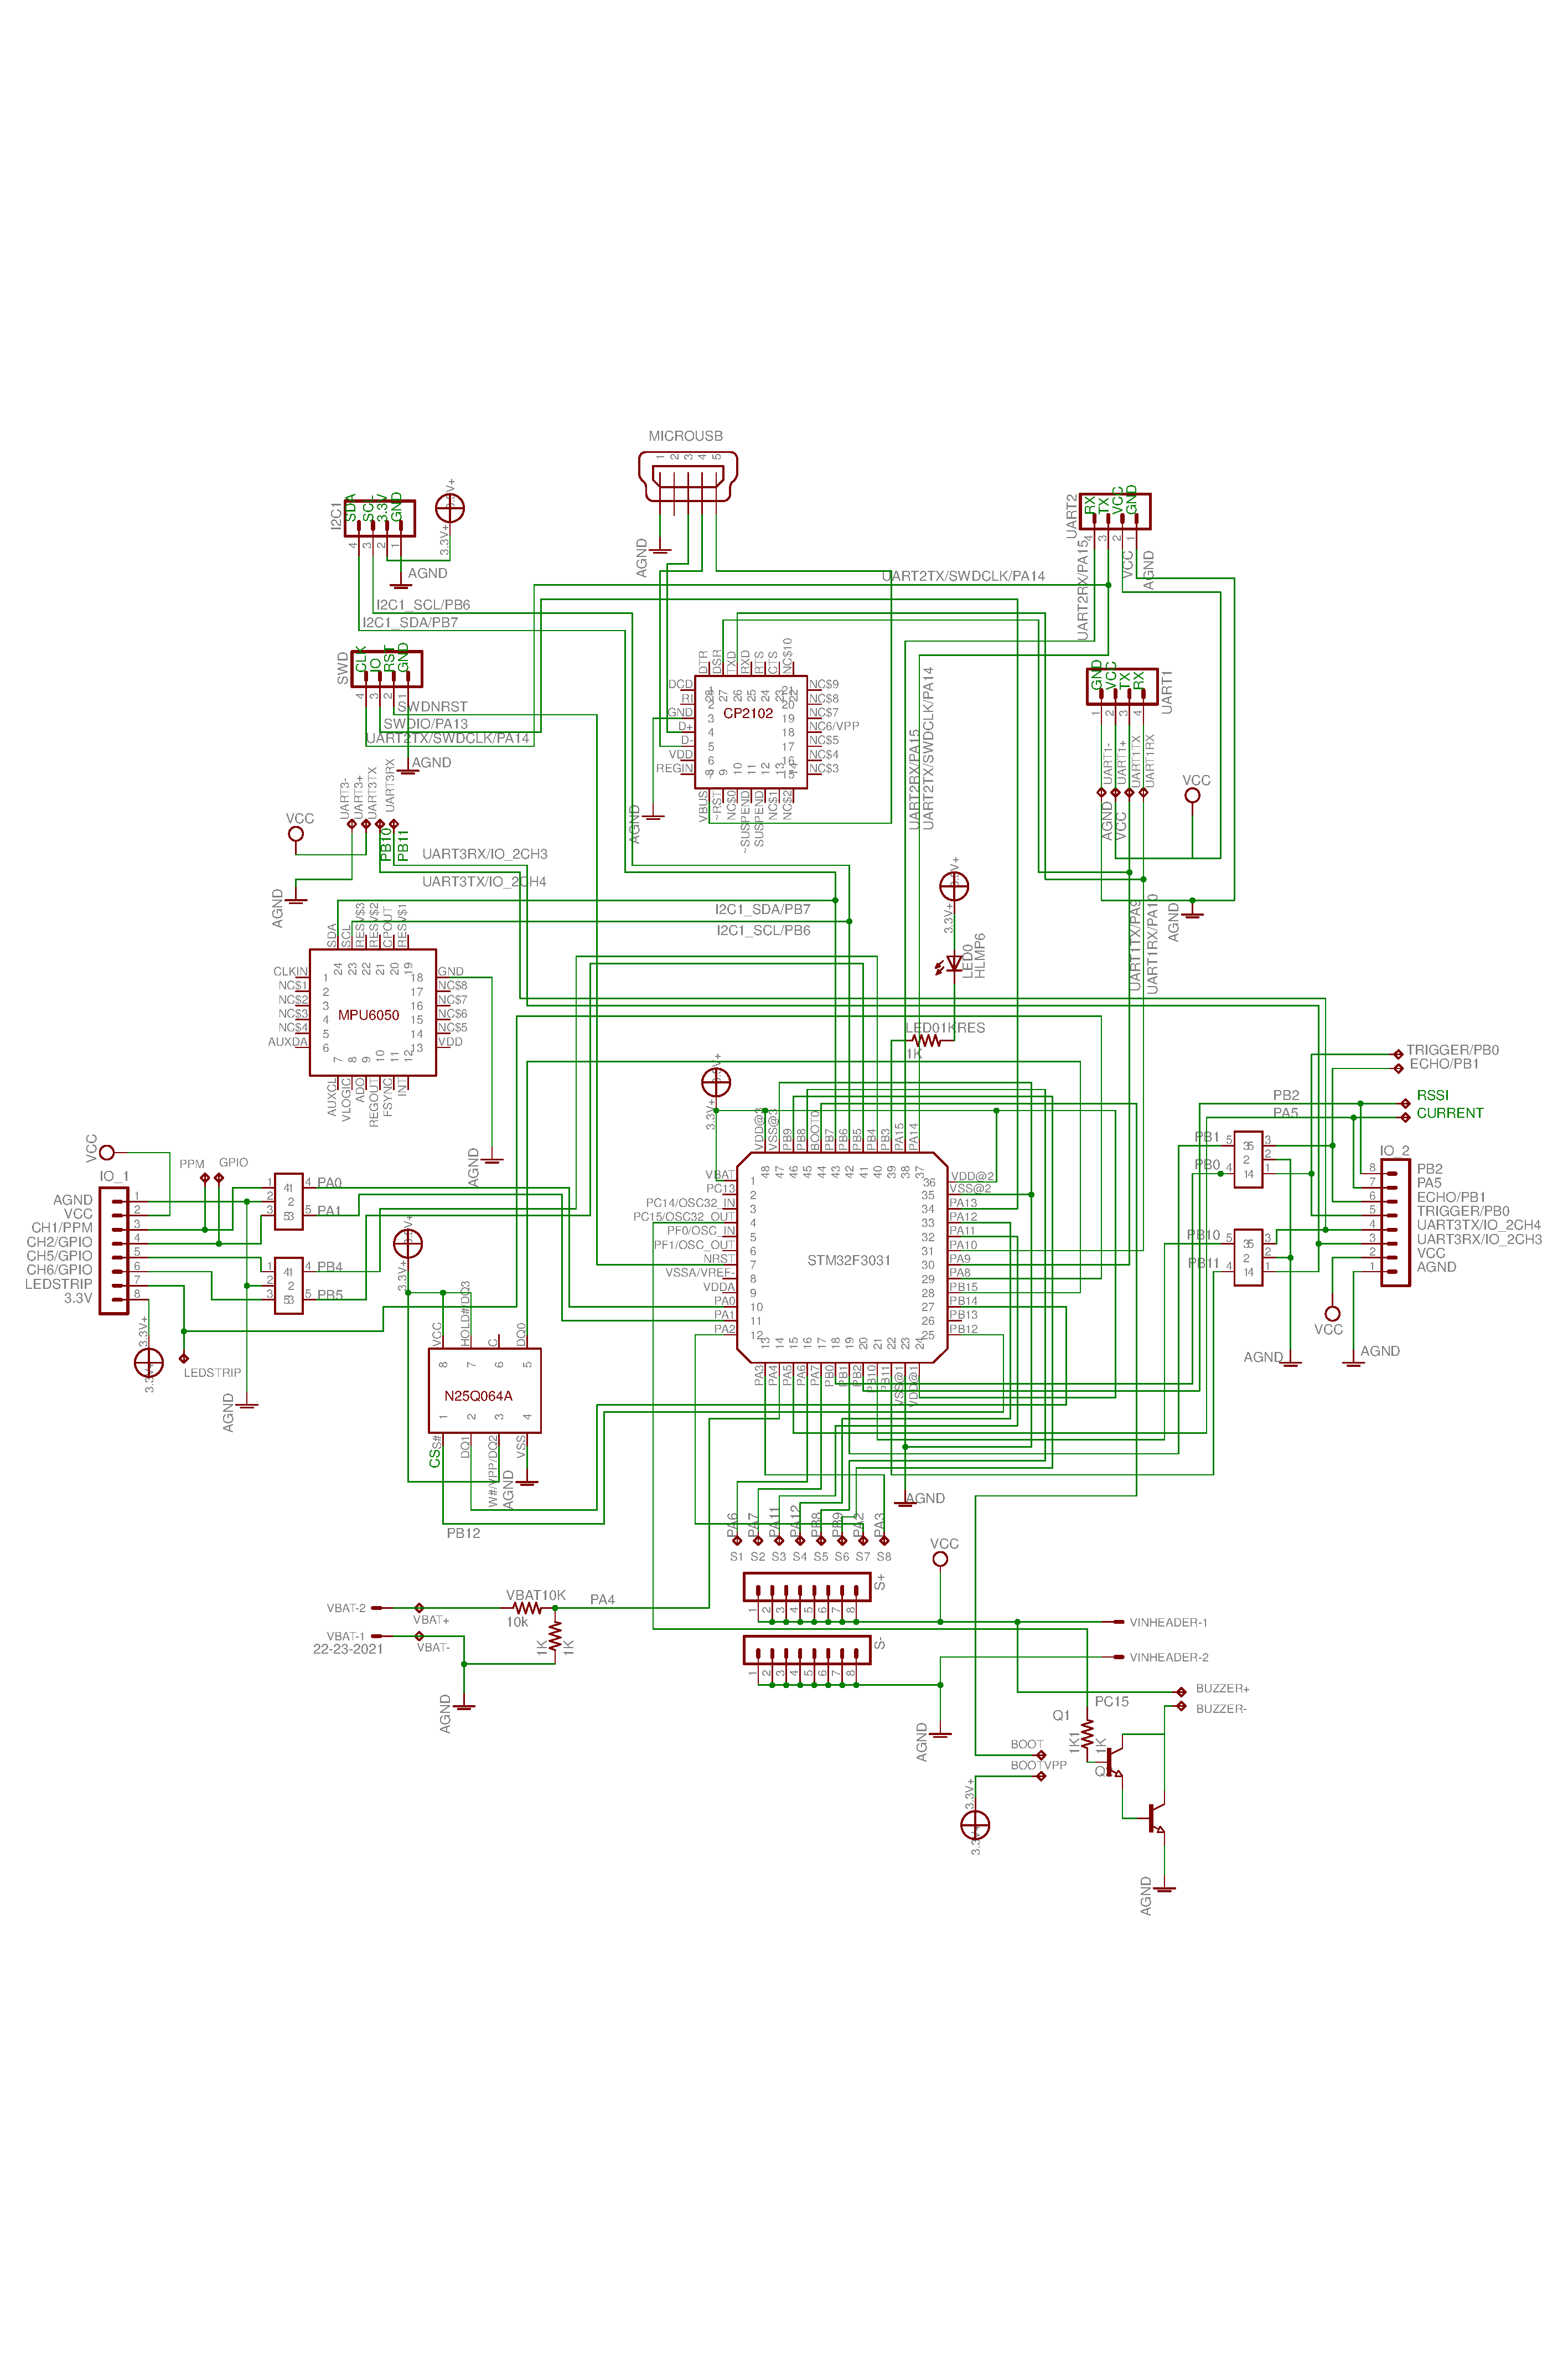
\includegraphics[width=\textwidth]{pdfpages/deluxe-schematic.pdf}
\end{minipage}
}
\captionof{figure}{F3 Deluxe Flight Controller Hardware Schematic}
}
\restoregeometry
%-----------------------------------------------------
\newpage
%-----------------------------------------------------
\newgeometry{left=1cm,right=1cm,top=2cm,bottom=1cm}
\section{Strain Gauge Amplification}
\label{app:strain}
{\centering
\fbox{
\begin{minipage}{0.9\textwidth}
\centering
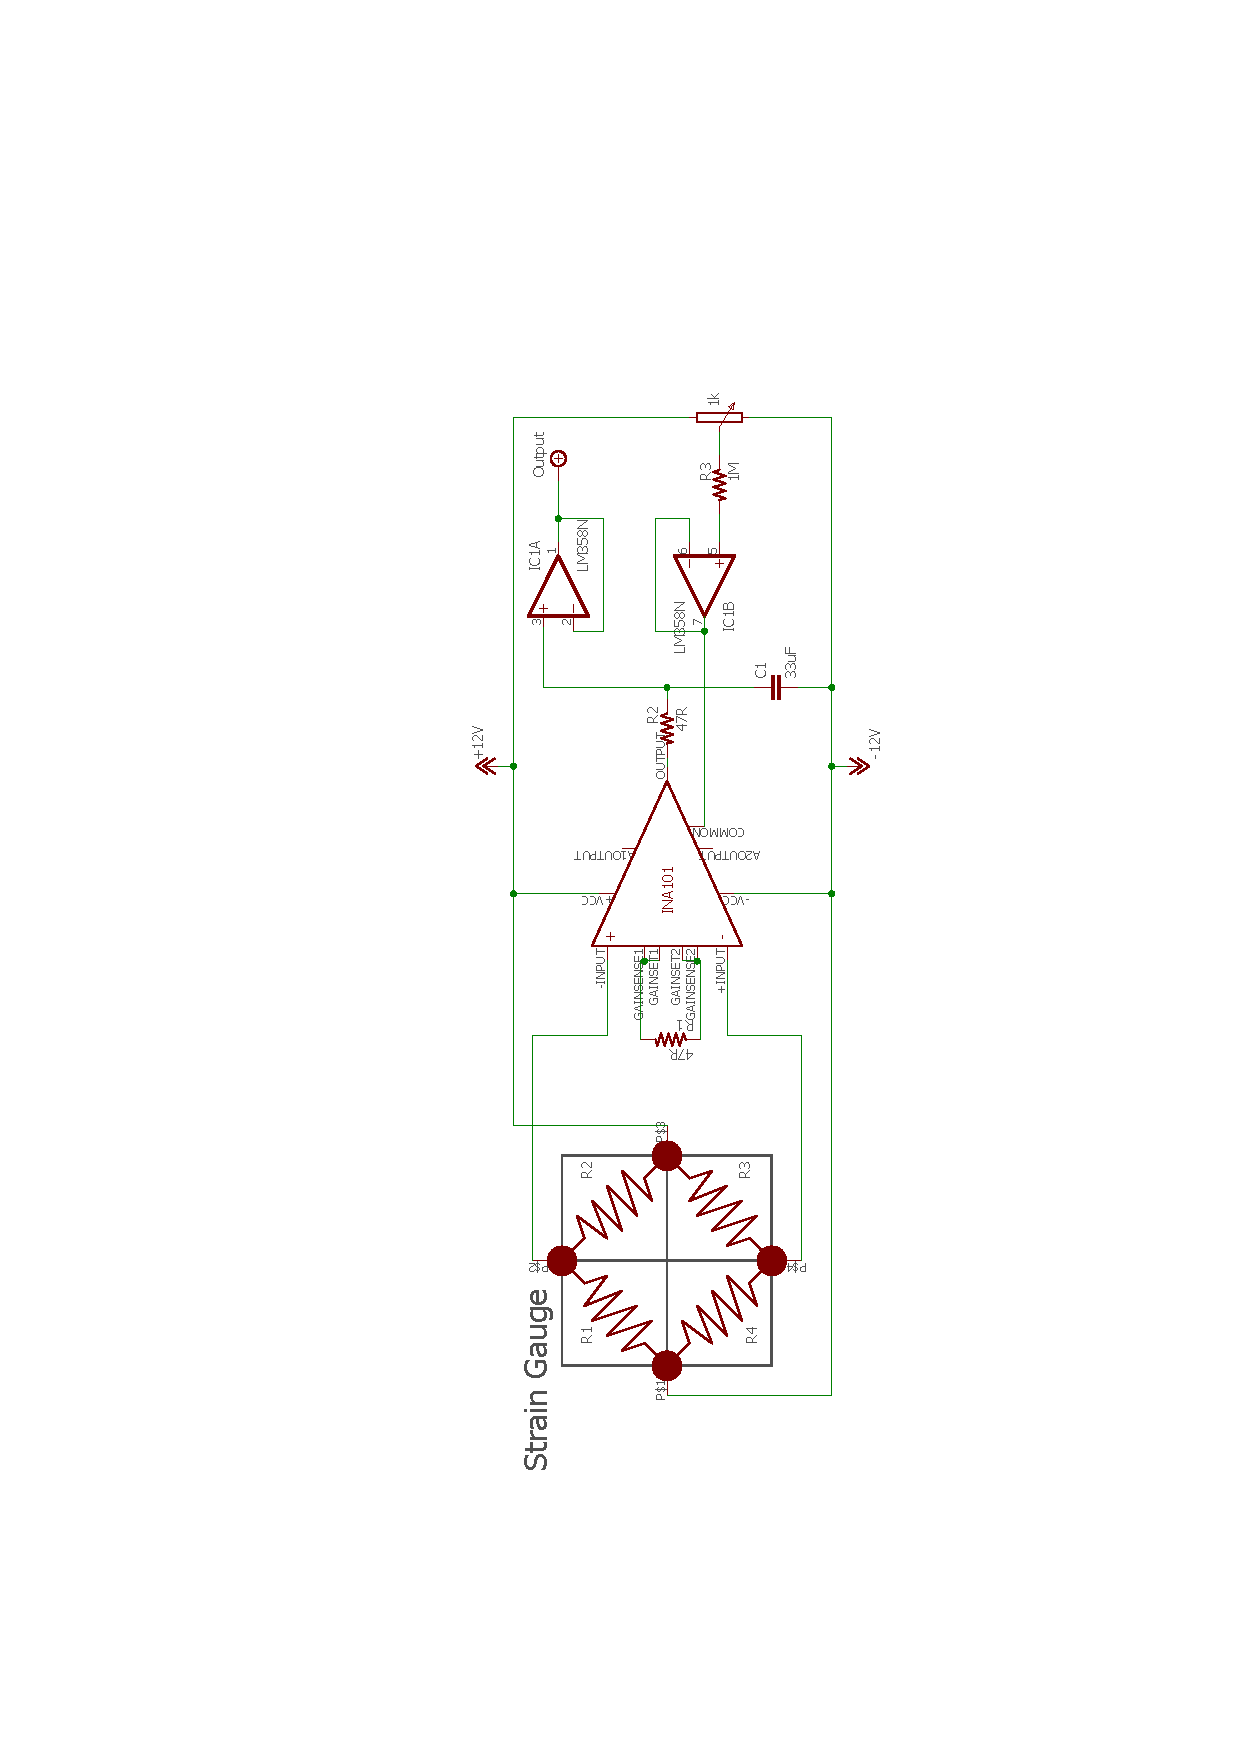
\includegraphics[clip,trim=7.5cm 4cm 5.5cm 6cm,angle=-90,width=\textwidth]{pdfpages/strain.pdf}
\end{minipage}
}
\captionof{figure}{Strain gauge full bridge amplifier}
}
\restoregeometry
%-----------------------------------------------------
\newpage
%-----------------------------------------------------
\chapter{System ID Test Data}
\label{app:systemdat}
%-----------------------------------------------------
\section{Thrust and Torque Test Data}
\label{app:thrust-torque}
%-----------------------------------------------------
\vspace{-20pt}
\begin{figure}[htbp]
\begin{subfigure}{0.5\textwidth}
\centering
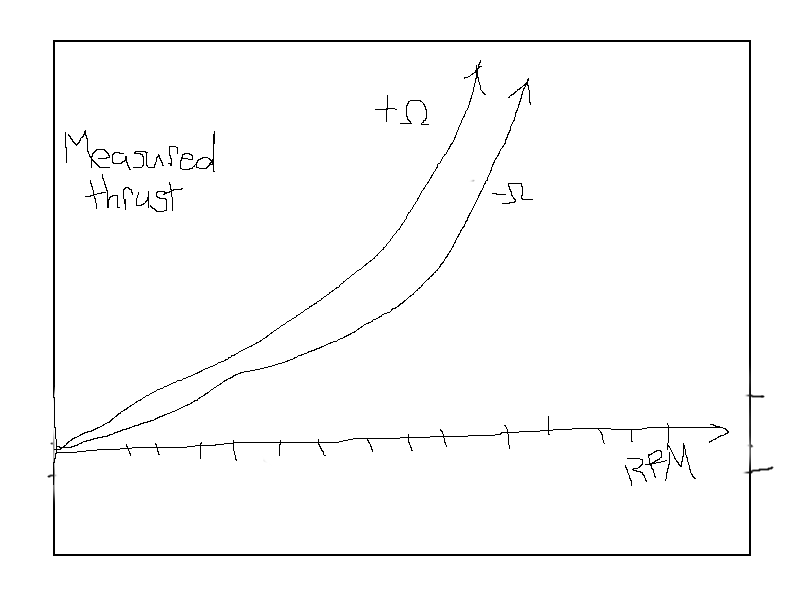
\includegraphics[width=\textwidth]{graphs/thrust-rotation}
\caption{Thrust tests}
\label{app:thrust-test}
\end{subfigure}
\begin{subfigure}{0.5\textwidth}
\centering
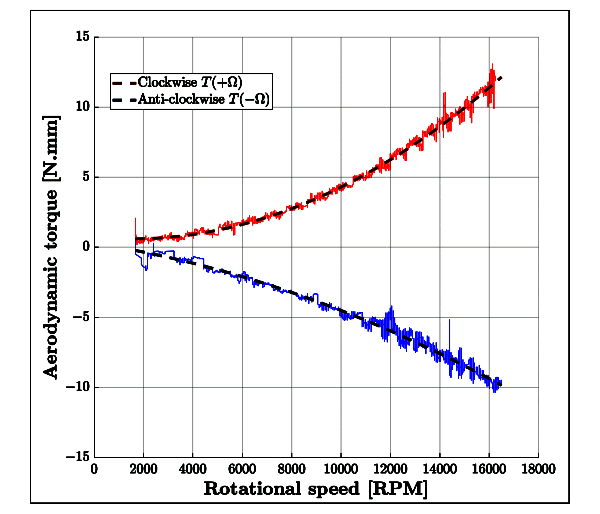
\includegraphics[width=\textwidth]{graphs/torque-rotation}
\caption{Torque tests}
\label{app:torque-test}
\end{subfigure}
\caption{Clockwise and counterclockwise rotation tests}
\end{figure}
Thrust tests in Fig:\ref{app:thrust-test} causes lateral deflection of the strain gauge thrust test rig illustrated in Fig:\ref{fig:thrust-rig}. The deflection is in the direction of the propeller's rotational sense, as a result of the torque applied to the propeller. Clockwise and counter-clockwise tests where summed together and averaged to produce the thrust tests plotted in Fig:\ref{fig:thrusts}.
\par
Torque tests in Fig:\ref{app:torque-test} shows thrust deflection in the rotational torque test rig in Fig:\ref{fig:torque-rig}. Upward thrust still resulted in some small deflection in the resultant measurements so opposing clockwise and counter-clockwise results were subtracted and averaged out to produce the torque tests plotted in Fig:\ref{fig:torques}.
\newpage
%-----------------------------------------------------
\newgeometry{left=1cm,right=1cm,top=2cm,bottom=1cm}
\section{Cobra CM2208-200KV Thrust Data}
\label{app:cobra-test}
\centering
\fbox{
\begin{minipage}{0.9\textwidth}
\centering
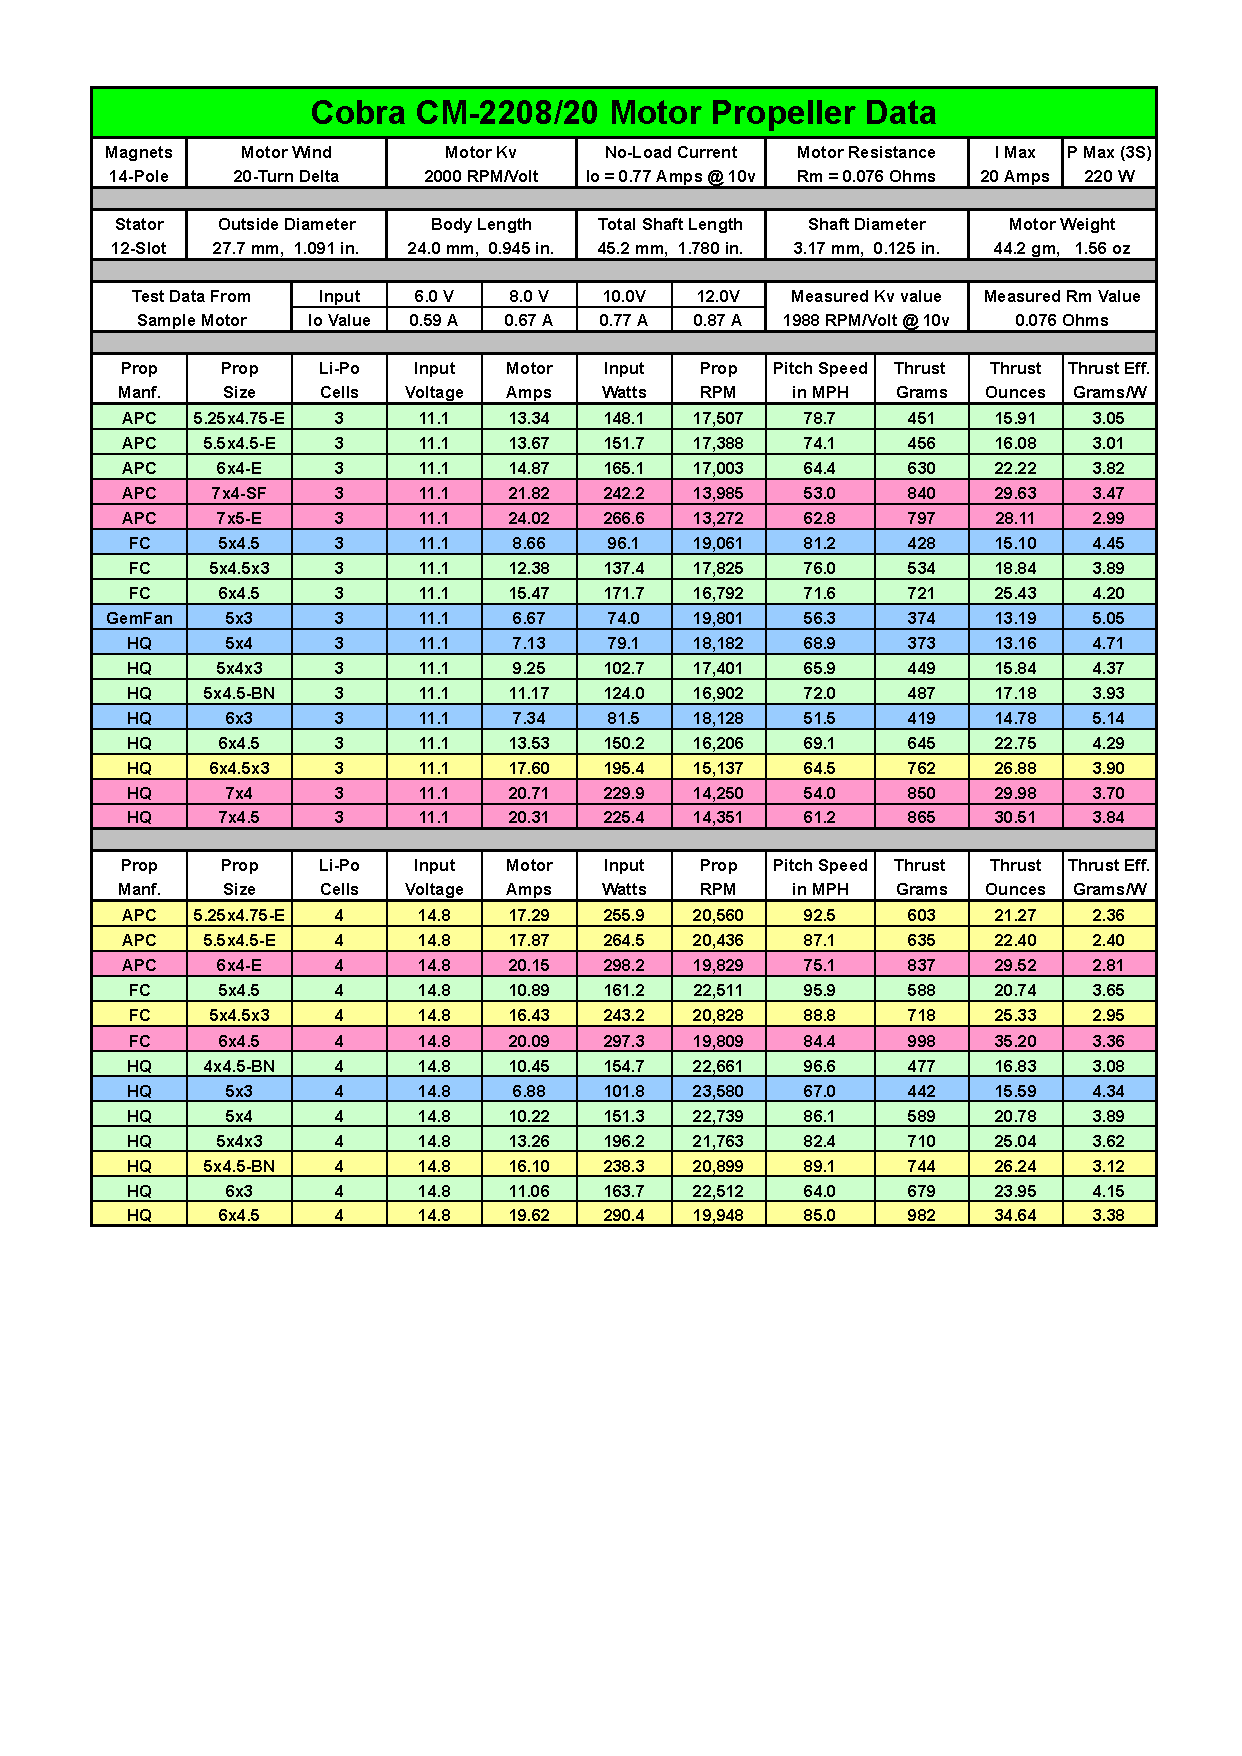
\includegraphics[width=\textwidth]{pdfpages/cobra-test.pdf}
\end{minipage}
}
\captionof{figure}{Official Test Results for Cobra Motors}
\restoregeometry
\newpage
\justifying
\parskip	= 10pt						% Paragraph spacing
\parindent 	= 0pt						% No para. indent
%-----------------------------------------------------
\section{Combined Simulated Torque Responses}
\label{app:tau-comb}
%-----------------------------------------------------
The process in Sec:\ref{subsec:dynamics.nonlinearities.torque-tests} applied simulation tests to the generalized torque responses derived in Sec:\ref{subsec:dynamics.nonlinearities.gyrotorques}. Previous simulations only considered separate singular perturbations in either $\lambda_i$ or $\alpha_i$ rotational positions alone. The generalized torque response $\vec{\mathbf{V}}(\alpha_i,\lambda_i)$, from Eq:\ref{eq:3.86g}, acts as a response to \emph{net motor module} rotations of both inner and middle ring servos $\lambda_i$ and $\alpha_i$ respectively.
\par
The plot in Fig:\ref{fig:tau-com-lambda} shows varying steps for $\Delta\lambda_i$ with a constant $\Delta\alpha_i=\pi/4$ step. The error between an estimated value $\hat{V}(\alpha_i,\lambda)$, with a linearized rotation partial derivative, and the true $\widetilde{V}(\alpha,\lambda)$ is shown in Fig:\ref{fig:tau-comb-lam-r}. That error is mostly of the order $\times 10^{-4}~[\text{N.m}]$; whilst both $\hat{V}(\alpha_i,\lambda_i)$ and $\widetilde{V}(\alpha_i,\lambda_i)$ are in the order of $\times 10^{-1}~[\text{N.m}]$.
\begin{figure}[htbp]
\vspace{-10pt}
\centering
\begin{subfigure}{0.49\textwidth}
\centering
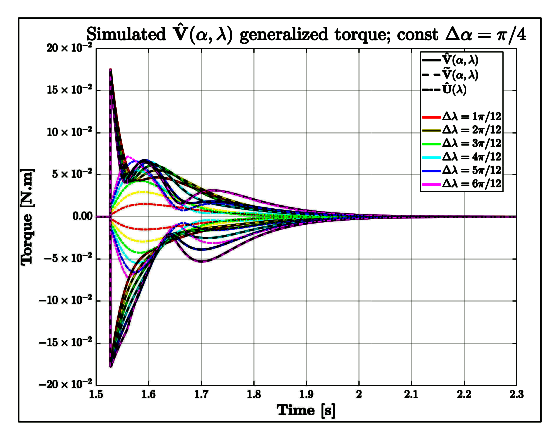
\includegraphics[width=\textwidth]{graphs/tau-comb-lam}
\caption{Torque response $\vec{\mathbf{V}}(\alpha_i,\lambda_i)$ to steps in $\Delta\lambda_i$ only}
\label{fig:tau-comb-lam}
\end{subfigure}
\begin{subfigure}{0.49\textwidth}
\centering
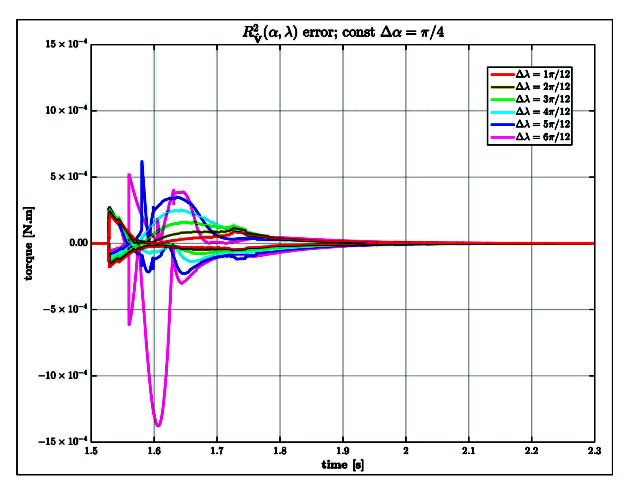
\includegraphics[width=\textwidth]{graphs/tau-comb-lam-r}
\caption{Error for $\vec{\mathbf{V}}(\alpha_i,\lambda_i)$ for steps in $\Delta\lambda_i$ only}
\label{fig:tau-comb-lam-r}
\end{subfigure}
\vspace{-6pt}
\caption{Step changes in $\Delta\lambda_i$ with constant $\Delta\alpha_i=\pi/4$}
\label{fig:tau-com-lambda}
\vspace{-16pt}
\end{figure}
\par
Similarly, Fig:\ref{fig:tau-comb-alph} shows the same tests run for varying step sizes of $\Delta\alpha_i$ with a constant step size for $\Delta\lambda_i=\pi/4$. Again, the plot Fig:\ref{fig:tau-comb-alph-r} shows the error which, on average, is in the order of $\times 10^{-4}~[\text{N.m}]$. The error between a simplified $\hat{V}(\alpha_i,\lambda_i)$ and the true $\widetilde{V}(\alpha_i,\lambda_i)$ only becomes significant as the step size $\Delta\alpha_i$ tends to $\pi/2$.
\begin{figure}[htbp]
\vspace{-10pt}
\centering
\begin{subfigure}{0.49\textwidth}
\centering
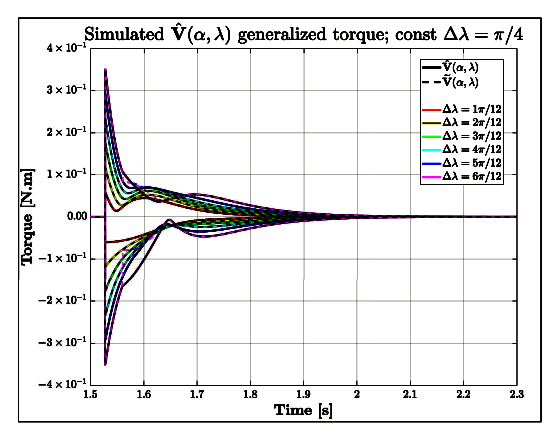
\includegraphics[width=\textwidth]{graphs/tau-comb-alph}
\caption{Torque response $\vec{\mathbf{V}}(\alpha_i,\lambda_i)$ to steps in $\Delta\alpha_i$ only}
\label{fig:tau-comb-alph}
\end{subfigure}
\begin{subfigure}{0.49\textwidth}
\centering
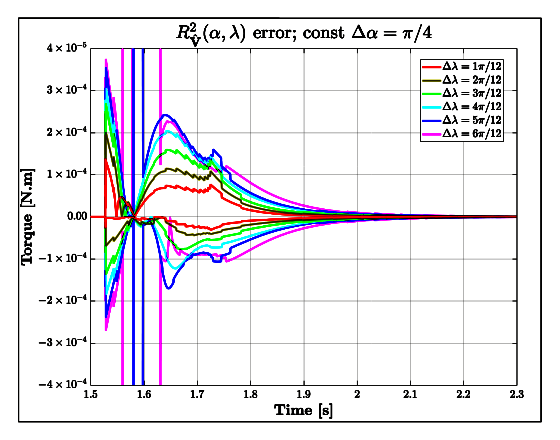
\includegraphics[width=\textwidth]{graphs/tau-comb-alph-r}
\caption{Error for $\vec{\mathbf{V}}(\alpha_i,\lambda_i)$ for steps in $\Delta\alpha_i$ only}
\label{fig:tau-comb-alph-r}
\end{subfigure}
\vspace{-6pt}
\caption{Step changes in $\Delta\alpha_i$ with constant $\Delta\lambda_i=\pi/4$}
\label{fig:tau-comb-alpha}
\vspace{-16pt}
\end{figure}
\par
It is interesting to note that positive and negative step directions are not symmetrical in their responses for Fig:\ref{fig:tau-comb-lam} and Fig:\ref{fig:tau-comb-alph}. This is as a result of the gyroscopic cross product in the calculations for $\hat{V}(\alpha_i,\lambda_i)$. Both tests shown in Fig:\ref{fig:tau-com-lambda} and Fig:\ref{fig:tau-comb-alpha} further corroborate the model proposed previously in Sec:\ref{subsec:dynamics.nonlinearities.gyrotorques}.
\newpage
%-----------------------------------------------------
\section{Controller Disturbance Rejection}
\label{app:disturbance}
%-----------------------------------------------------
\subsection{Attitude Controllers}
\label{app:disturbance.attitude}
%-----------------------------------------------------
\begin{figure}[htbp]
\centering
\begin{subfigure}{\textwidth}
\vspace{-12pt}
\centering
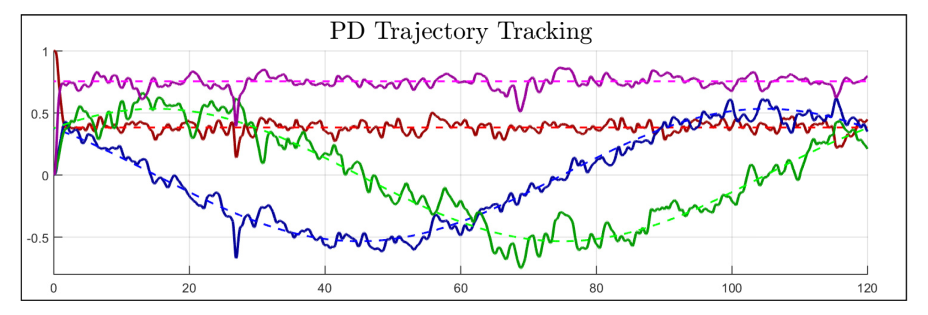
\includegraphics[width=0.8\textwidth]{graphs/PD_Diagonal_Trajectory_dist}
\vspace{-12pt}
\caption{Diagonal Proportional Derivative Controller}
\label{fig:app-attitude-pd-dist}
\end{subfigure}
\begin{subfigure}{\textwidth}
\vspace{-3pt}
\centering
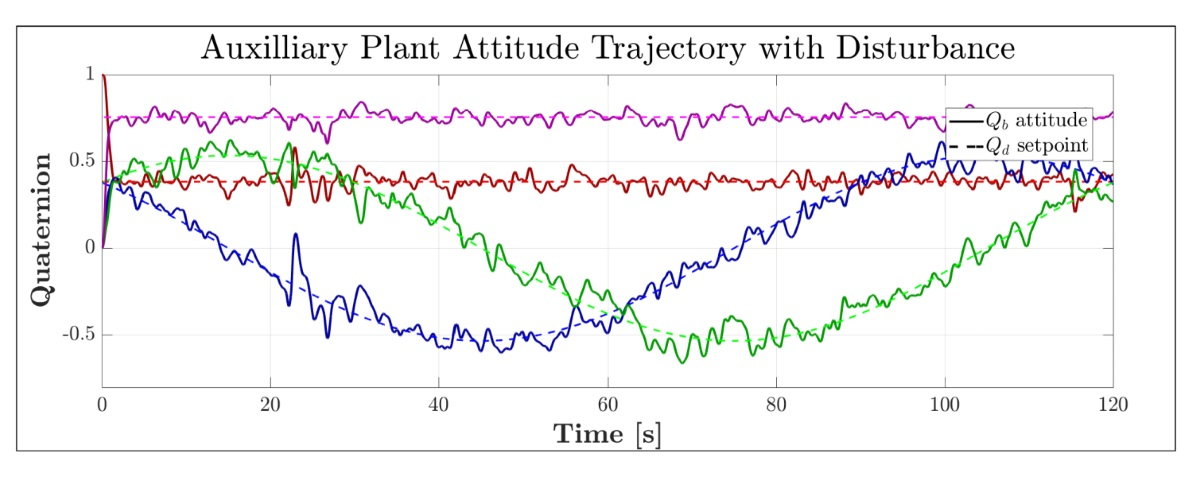
\includegraphics[width=0.8\textwidth]{graphs/XPD_Trajectory_dist}
\vspace{-12pt}
\caption{Auxilliary Plant Controller}
\label{fig:app-attitude-xpd-dist}
\end{subfigure}
\begin{subfigure}{\textwidth}
\vspace{-3pt}
\centering
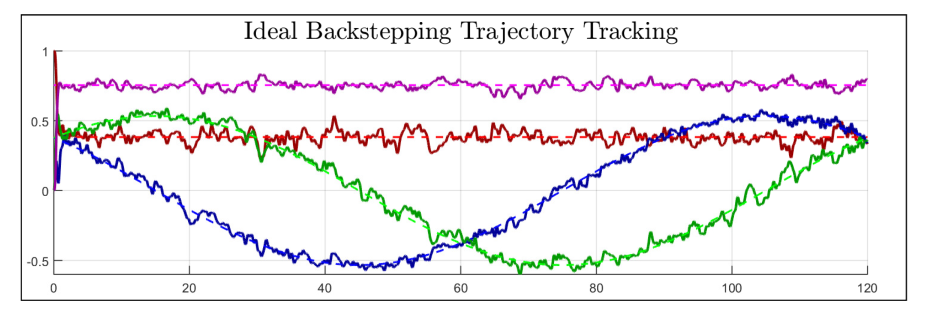
\includegraphics[width=0.8\textwidth]{graphs/IBC_Trajectory_dist}
\vspace{-10pt}
\caption{Ideal Backstepping Controller}
\label{fig:app-attitude-ibc-dist}
\end{subfigure}
\vspace{-3pt}
\caption{Disturbances on Attitude Controllers}
\end{figure}
\newpage
%-----------------------------------------------------
\subsection{Position Controllers}
\label{app:disturbance.position}
%-----------------------------------------------------
\begin{figure}[htbp]
\centering
\begin{subfigure}{\textwidth}
\vspace{-12pt}
\centering
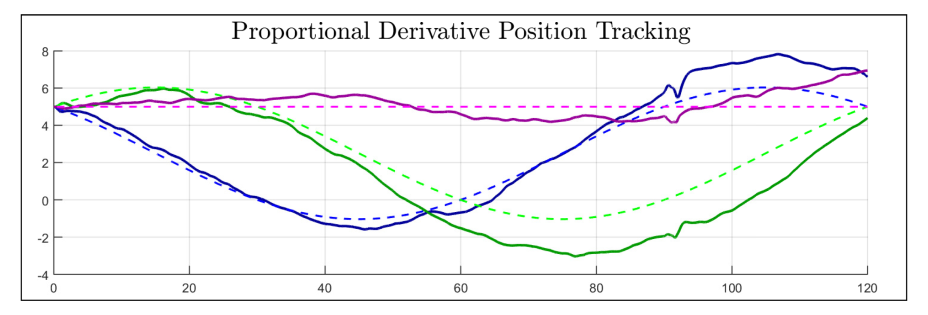
\includegraphics[width=0.8\textwidth]{graphs/PD_Position_Trajectory_dist}
\vspace{-12pt}
\caption{Proportional Derivative Controller}
\label{fig:app-position-pd-dist}
\end{subfigure}
\begin{subfigure}{\textwidth}
\vspace{-3pt}
\centering
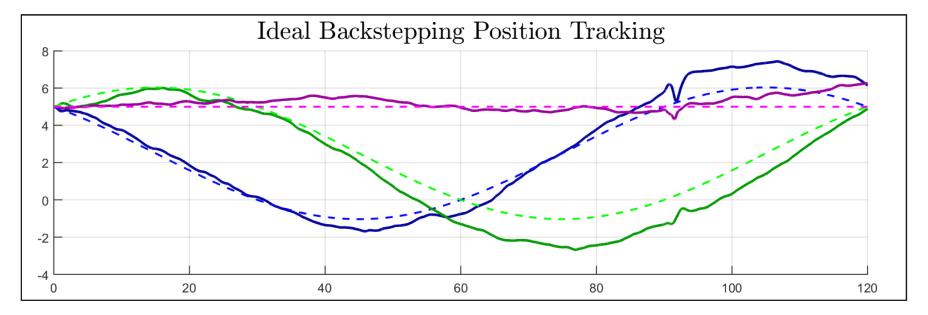
\includegraphics[width=0.8\textwidth]{graphs/IBC_Position_Trajectory_dist}
\vspace{-12pt}
\caption{Ideal Backstepping Controller}
\label{fig:app-position-ibc-dist}
\end{subfigure}
\caption{Disturbances on Position Controllers}
\end{figure}